\chapter[Giant Number Fluctuations in 3-Dimensional Space]{Giant Number Fluctuations in 3-Dimensional Space}
\label{giant-number-fluctuations-in-3-dimensional-space}
%%%%%%%%%%%%%%%%%%%%%%%%%%%%%%%%%%%%%%%%%%%%%%%%%%%%%

\section{Introduction}
Active fluids exhibit many unusual behaviors beyond the expectation of equilibrium statistical mechanics \cite{Ramaswamy2010,Cates2012,Marchetti2013,Poon2013,Elgeti2015}.
In particular, an active fluid can exhibit anomalously large density variations, the so-called giant number fluctuations (GNF), where the standard deviation of the number of particles grows nonlinearly with the square root of the mean particle number, defying the central limit theorem of equilibrium systems \cite{Mishin2015}.
Such unusual density fluctuations have been observed in a wide range of active fluids in both living and non-living systems including vibrated granular rods \cite{Narayan2007,Aranson2008,Kudrolli2008,Deseigne2010},
swarming bacteria \cite{Zhang2010,Nishiguchi2017} and mammalian cells \cite{Kawaguchi2017},
self-propelled cytoskeleton \cite{Schaller2013}, and synthetic colloidal swimmers \cite{Palacci2013,Karani2019}. As a result, GNF has generally been viewed as a hallmark of the emergent behaviors of active fluids.


Significant theoretical and computational advancement on GNF has been made over the past two decades since the seminal works of Toner and Tu \cite{Toner1995,Tu1998,Toner1998,Simha2002,Ramaswamy2003,Toner2005,Chate2008,Mishra2010,
Dey2012,Saintillan2012,Saintillan2013,Ngo2014,Mahault2019}. Meanwhile, many important theoretical and numerical predictions have been tested in experimental realizations
\cite{Narayan2007, Aranson2008, Deseigne2010, Zhang2010, Schaller2013,
Nishiguchi2017, Kawaguchi2017, Palacci2013}.

Of particular interest is the scaling exponent $\alpha$, which is defined following $\Delta N /\sqrt N \propto N^\alpha$, where $\Delta N$ is the standard deviation of particle number and $N$ is the mean number of particles in a subsystem of given size. Heretofore, all the existing experiments on GNF were limited to two-dimensional (2D) or quasi-2D systems. In contrast to theoretical predictions (where $\alpha \approx 0.3$), $\alpha$'s obtained in these experiments show large variations ranging from 0.13 to 0.5. Such a large variation arises partially because of complicated particle-boundary interactions, which are hard to incorporate in theoretical studies. Moreover, the predictions of $\alpha$ in three-dimensional (3D) wet active fluids---one of the most important classes of active fluids where hydrodynamics dominate the interparticle interactions and conserve the total momentum of systems \cite{Marchetti2013}---has not been experimentally testified. Therefore, there is an imperative need for an experimental measurement of $\alpha$ in 3D active fluids, which are not affected by system boundaries. Such a measurement will provide not only an unambiguous experimental benchmark to testify theories of active fluids, but also experimental support on the effect of dimensionality on GNF of active fluids \cite{Marchetti2013}.

The rise of GNF in active fluids is usually accompanied by the transition to ordered phases with collective motions \cite{Ramaswamy2010,Marchetti2013}. For wet 3D active fluids such as bacterial suspensions, these collective motions lead to large-scale coherent flows with intermittent vortices and jets, which are often referred to as active turbulence \cite{Wolgemuth2008,Wensink2012,Dunkel2013a,Bratanov2015,Guo2018,Linkmann2019,Bardfalvy2019,Alert2020,Skultety2020,Peng2020}. Similar to GNF that manifests density fluctuations across different scales, the flow of active turbulence also exhibits scale-dependent structures.
Imported from the study of classical turbulence, energy spectra are frequently measured to quantify such structures in active turbulence \cite{Ishikawa2011,Wensink2012,Dunkel2013a,Giomi2015,Creppy2015,Patteson2018,Alert2020}. Although both GNF and energy spectra quantify the scale-dependent dynamics of active fluids, the deep connection between these two quantities at different scales has not been experimentally investigated. Our experiment reveals the density- and scale- independent coupling between GNF and energy spectra, suggesting that GNF is governed by the strength of the motion-induced flow.

\begin{figure}[!htbp]
\begin{center}
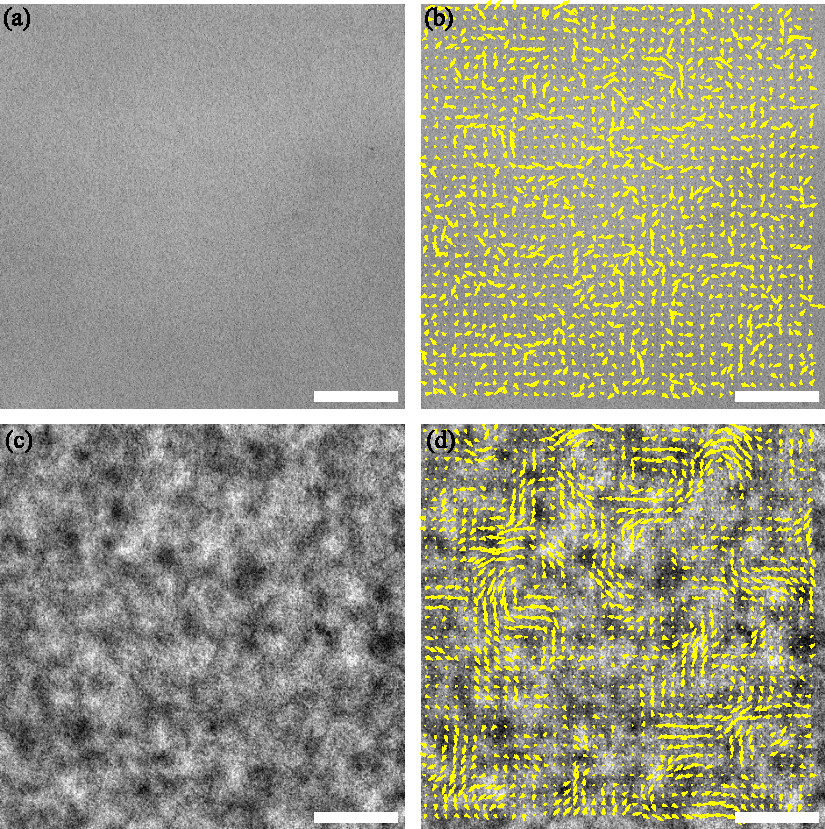
\includegraphics[width=5.5in]{figs/5-GNF/1.pdf}
\caption[Images of Bacterial Active Turbulence and Its Flow Fields]
{
\textbf{Images of bacterial active turbulence and its flow fields.}
(a) and (b) are active turbulence in a dense bacterial suspension (1.6\%) displaying constantly varying concentration inhomogeneity and the corresponding flow field.
(c) and (d) are a dilute bacterial suspension (6.4\%) and the corresponding flow field.
Scale bars are 85 $\mu$ m.
}
\label{fig:experiment}
\end{center}
\end{figure}


\section{Methods}

\subsection{Sample Preparation, Imaging and Analysis}
Here, we present our systematic experimental study of GNF and energy spectra in bulk bacterial suspensions, a premier example of 3D wet active fluids. We use genetically engineered light-powered \textit{Escherichia coli} (\textit{E. coli}) as our model bacteria.
For a typical experiment, a bacterial suspension of control volume fraction $\phi$ is injected into a sealed chamber of 20 mm $\times$ 3 mm $\times$ 140 $\mu$m.
Without supply of oxygen, bacteria quickly consume all the remaining oxygen in the chamber and stop moving after $5$ minutes.
We then illuminate the suspension with a high-intensity microscope light, which powers bacteria at their maximal swimming speed of $15 \pm 3$ $\mu$m/s in the dilute limit.
A video of the suspension is taken 50 $\mu$m above the bottom wall of the chamber by a bright-field inverted microscope at a frame rate of $30$ fps and the field of view of $420 \times 360$ $\mu$m$^2$ (Fig.~\ref{fig:experiment}a, c).
We use a standard Particle Image Velocimetry (PIV) algorithm \cite{OpenPIV-website}
to extract the 2D in-plane velocity field $(v_x,v_y)$ in the 3D suspension, which exhibits the characteristic chaotically-moving vortices and jets of active turbulence at high $\phi$ (Fig.~\ref{fig:experiment}b, d).

\subsection{The Relation between Pixel Intensity and Concentration}

It is challenging to directly count the number of bacteria in a 3D suspension of fasting moving bacteria. Luckily, by virtue of Beer-Lambert law, the local bacterial density is monotonically correlated with the local intensity of microscope images, where darker regions correspond to higher bacterial densities (Fig.~\ref{fig:experiment}c). Similarly principles also appeared in other experimental works, where optical information was exploited in probing the dynamics in suspensions of bacteria and actin filaments \cite{Sokolov2009, Wilson2011, Schaller2013}.

\begin{figure}[!htbp]
\begin{center}
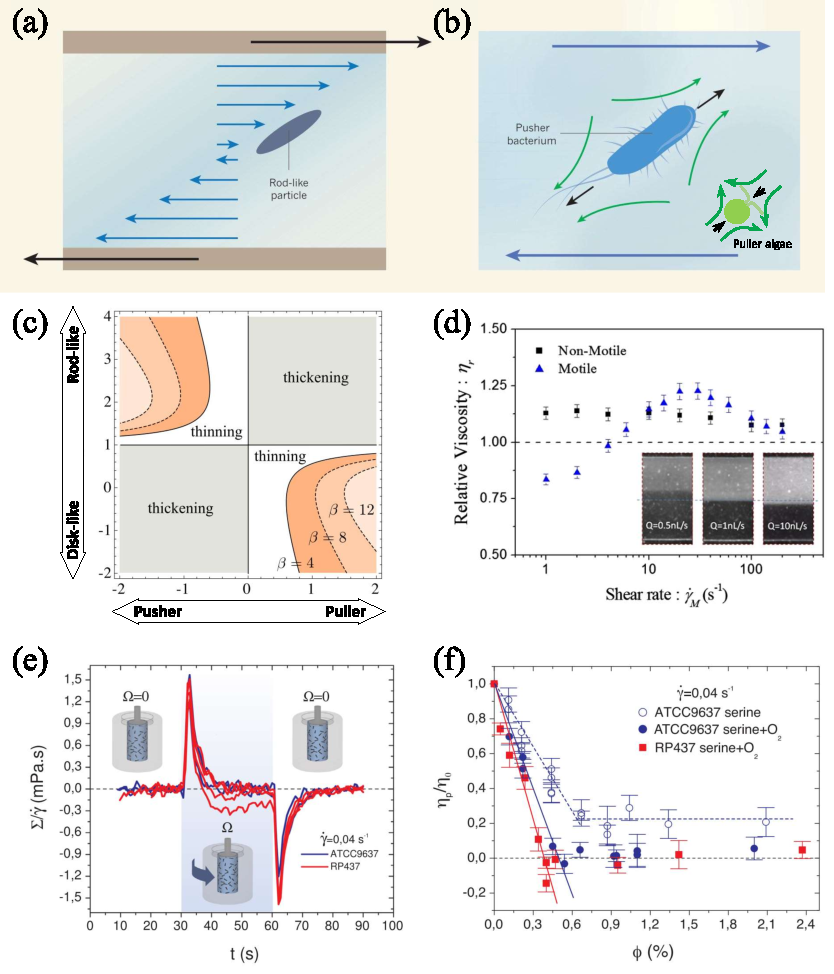
\includegraphics[width=3.5in]{figs/5-GNF/2.pdf}
\caption[Relation between Image Intensity and Concentration]
{
\textbf{Relation between image intensity and concentration.}
(a) Images of bacterial suspensions of different volume fractions under the same illumination conditions.
(b) Volume fractions as a function of average pixel intensities.
}
\label{fig:calibration}
\end{center}
\end{figure}

To calibrate the density-intensity correlation, we prepare bacterial suspensions of different $\phi$ and image the suspensions under the same illumination (Fig.~\ref{fig:calibration}a). The mean image intensity decreases with increasing $\phi$ following an approximately linear relation (Fig.~\ref{fig:calibration}b), agreeing with the Beer-Lambert law for samples of small thickness and weak absorptivity appropriate for our experiments. The linear density-intensity relation has also been used in previous experiments on \textit{E. coli} suspensions \cite{Wilson2011}.

In the low attenuation limit (small thickness and weak absorptivity), $I=I_0-\epsilon$ where $\epsilon\ll I_0$:
\begin{equation}
  \log \frac{I_0}{I} = \log \frac{I_0}{I_0 - \epsilon} \approx \frac{\epsilon}{I_0} \sim c
\end{equation}
\begin{equation}
I = I_0 - \epsilon \sim c
\end{equation}
where $I_0$ is the original light intensity, $I$ is the transmission light intensity, $\epsilon$ is the attenuated light intensity, which is much smaller than the original light intensity.

\begin{figure}[!htbp]
\begin{center}
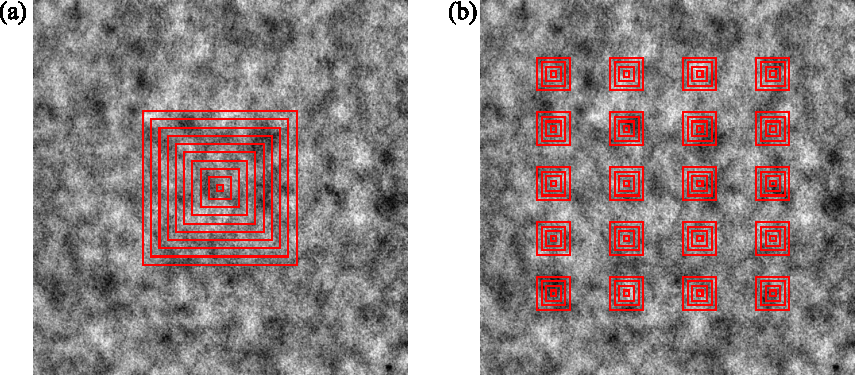
\includegraphics[width=0.9\textwidth]{figs/5-GNF/GNF-calculations.pdf}
\caption[GNF Calculations]
{
\textbf{GNF calculations.}
(a) Varying subsystem sizes.
(b) Multiple seeds of subsystems for spatial average.
}
\label{GNF-calculation}
\end{center}
\end{figure}

\subsection{GNF Calculations}
In Fig.~\ref{fig:calibration}b, we show that under the same illumination and imaging condition, bacterial density and the average pixel intensity follow approximately a linear relation, which can be expressed as follows:
\begin{equation}
\label{eq:phi-I-relation}
\phi = a + bI,
\end{equation}
where $\phi$ is the volume fraction of bacterial suspensions, $I$ is the average pixel intensity, $a$ and $b$ are constants at the fixed illumination and imaging condition. The number of bacteria in a given subsystem of side length $l$ and thickness $d$ can be calculated as
\begin{equation}
\label{eq:n}
N = \frac{l^2d}{V_b} \phi = \frac{l^2d}{V_b} (a+bI),
\end{equation}
where $V_b$ is the volume of a single bacterium. $d \approx 6$ $\mu$m is the depth of the field of microscopy, which is fixed in our experiments. Thus, the number of bacteria in the subsystem $N$ is proportional to $l^2 \phi$. Taking the standard deviation of both sides of Eq.~\ref{eq:n}, we obtain
\begin{equation}
\label{intensity-number}
\Delta N = \frac{l^2 d}{V_b}|b|\Delta I,
\end{equation}
where $\Delta N$ is the standard deviation of the bacterial number in the subsystem over time and $\Delta I$ is the standard deviation of the average pixel intensity of the subsystem over time. Since $d|b|/V_b$ is a constant independent of subsystem sizes and bacterial volume fractions, $\Delta N$ is linearly proportional to $l^2\Delta I$. Because any constant in front of $\Delta N$ would not affect either the scaling relation or the relative magnitude of density fluctuations at different $\phi$, we simply take $l^2\Delta I$ as $\Delta N$ in our study.

Based on the linear relation between $\Delta N$ and $\Delta I$, we calculate the density fluctuations at different length scales. We first crop square-shape subsystems of increasing sizes, as shown in Fig.~\ref{GNF-calculation}. For each subsystem size $l$, the standard deviation of the average pixel intensity of the subsystem is calculated over 50 frames (1.67 s or 8.35$\tau_b$), which is longer than the saturated density correlation time of $4\tau_b = 0.8$ s. To improve statistics, we choose 20 subsystems of the same size evenly distributed in the field of view and obtain a spatial average of the temporal standard deviation of the average pixel intensity $\Delta I$ (Fig.~\ref{GNF-calculation}). This averaged $\Delta I$ is then multiplied by $l^2$ to give the number density fluctuations $\Delta N$ at the length scale $l$. Note that a second method has also been proposed for calculating number fluctuations, where the standard deviation of particle numbers is computed first spatially over different locations in a single time frame and is then averaged over time of different frames \cite{Aranson2008}.  Although the two methods lead to the same results when spatial and temporal correlations are small compared with the system size and experiment duration \cite{Aranson2008}, the second method is subject to potential systematic errors in our study due to time-independent non-uniform light illumination and intrinsic stationary density variations in non-motile suspensions at $t=0$ in the kinetic measurements. Using the first method, any stable non-uniform light illumination or stationary non-uniform density variations would result in zero temporal standard deviations of $I$ and, therefore, would not affect our measurements of true density fluctuations of motile bacterial suspensions.


\subsection{Normalization of GNF at Different Volume Fractions}

Practically, to optimize image qualities, we adjust the exposure time of imaging for suspensions of different $\phi$. Exposure times affect the proportional constant $b$ in Eq.~\ref{eq:phi-I-relation}, which introduces a $\phi$-dependent linear constant $b(\phi)$ in Eq.~\ref{eq:n}. Although $b(\phi)$ does not affect the scaling exponent of density fluctuations $\alpha$, it modifies the relative magnitude of $\Delta N$ at different $\phi$. In order to compare the magnitude of density fluctuations at different $\phi$,  we further calibrate and normalize $\Delta I$ for different $\phi$. Specifically, as the calibration, we take videos of bacterial suspensions at different $\phi$ under the exact same imaging condition with fixed illumination light intensity, condenser position, optical filters and all the camera settings such as the exposure time and the dynamic range. The calibration results are shown in Fig.~\ref{fig:same-conditions}, where $\Delta N \sim l^2 \Delta I$ at different $\phi$ collapse at small length scales. The calibration results show that we can normalize $l^2 \Delta I$ of different exposure times by its value at a fixed small length scale. We choose the small scale at $l = 0.3l_b$ in our study. Since $l^2 \Delta I$ at different $\phi$ shows the same slope at small $l$, choosing any other small lengths between $0.1l_b$ and $0.5l_b$ would lead to quantitatively the same results. The normalized density fluctuations show not only the correct scaling exponents but also the right relative magnitudes at different $\phi$.

\begin{figure}[!htbp]
  \begin{center}
    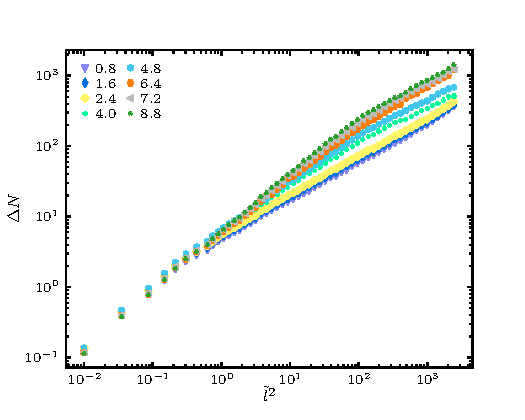
\includegraphics[width=4.5in]{Figs/5-GNF/GNF-normalization.pdf}
    \caption[Normalization of GNF at Different Volume Fractions]
    {
    Calibration of the standard deviation of bacterial number $\Delta N \sim l^2\Delta I$ at different volume fractions $\phi$. $\Delta N$ versus the dimensionless subsystem size $\tilde{l}^2 = l^2/l_b^2$ for bacterial suspensions at different $\phi$. The images are taking under the same illumination with the same imaging condition.
    }
    \label{fig:same-conditions}
  \end{center}
\end{figure}

\subsection{Correlation of Local Density Fluctuations and Kinetic Energies}

To calculate local temporal density fluctuations, we need to approximate instantaneous intensity variations. On the one hand, the time interval for calculating the intensity difference between two frames needs to be smaller than the density correlation time ($4\tau_b = 0.8$ s) in order to satisfy the instantaneous approximation. On the other hand, the time interval should be sufficiently long to suppress the influence of random fluctuations of image intensities in adjacent frames. In our study, we choose 0.3 s (10 frames) for the local density fluctuation calculation. We do not expect the results to be much different when varying this number from 0.17 to 0.6 s.

To calculate the local density variations at the length scale of $l = 2.75l_b$ and time $t$, we take 10 consecutive frames following the frame at $t$. All the 10 frames are first coarse-grained by averaging the intensity of pixels in square windows of size $2.75l_b \times 2.75l_b$ into single coarse-grained pixels (Fig.~\ref{fig:coupling-calculation}b). We then take the temporal standard deviation of the coarse-grained pixel intensity over the 10 frames at different positions to obtain a field of density fluctuations at $t$, $\delta N(\bm{r},t)$, as shown in Fig.~\ref{fig:coupling-calculation}d.

Independently, the PIV algorithm is also applied on the original images of the first two frames to obtain the velocity field at time $t$, $\bm{v}(\bm{r},t)$ (Fig.~\ref{fig:coupling-calculation}c). Since the step size of the PIV analysis is also at $2.75l_b$, the velocity field has the same dimensions as the coarse-grained density fluctuation field obtained above. The local kinetic energy can then be calculated as $E(\bm{r},t)=|\bm{v}(\bm{r},t)|^2/2$ (Fig.~\ref{fig:coupling-calculation}e). Finally, the normalized correlation between $\delta N(\bm{r},t)$ and $E(\bm{r},t)$ is computed as
\begin{equation}
C_s = \frac{\langle(\Delta N-\overline{\Delta N})(E-\overline{E})\rangle}{\sigma_{\Delta N}\sigma_{E}},
\end{equation}
where $\bar A$ indicates the mean of variable $A$, $\sigma_A$ indicates the standard deviation of $A$, and $\langle A \rangle$ denotes the average of $A$ over all the positions. The correlation quantifies the spatial similarity between $\delta N$ and $E$, which ranges between $-1$ to 1.

\begin{figure}[!htbp]
	\begin{center}
		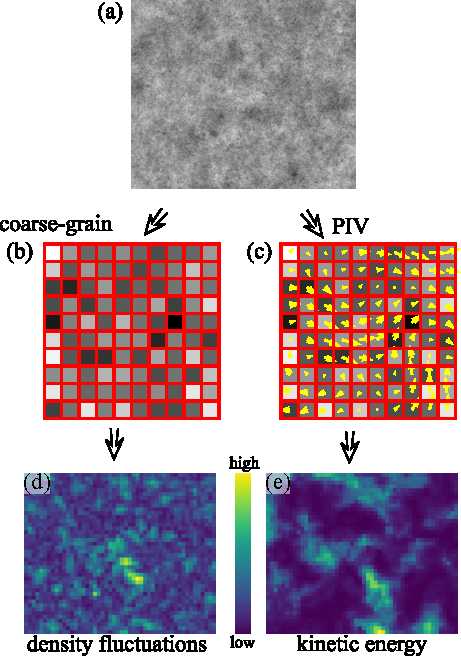
\includegraphics[width=3.5in]{Figs/5-GNF/local-correlation.pdf}
		\caption[Local Correlation between Density Fluctuations and Kinetic Energies]
		{
			Diagram showing the procedure to calculate the correlation between local density fluctuations and kinetic energies. (a) The raw image of a bacterial suspension at a given time $t$. (b) The coarse-grained image with a pixel size of $l=2.75l_b$. (c) The velocity field from PIV. (d) The field of local density fluctuations, obtained by calculating the standard deviation of the intensity of coarse-grained pixels shown in (b) over a short time interval. (e) The field of local kinetic energy, obtained by calculating $E = \bm{v}^2/2$ from the velocity field shown in (c).
 		}
		\label{fig:coupling-calculation}
	\end{center}
\end{figure}


\section{Results}
\subsection{Density Fluctuations}

The simple linear relation allows us to measure the spatiotemporal evolution of relative local bacterial densities and investigate density fluctuations in 3D bacterial suspensions. We first calculate the two-point density spatial correlation and the density auto-correlation for suspensions of different $\phi$ and compare them with well-studied velocity correlations extracted from PIV (Fig.~\ref{fig:spatiotemporal-correlations}).

\begin{figure}[!p]
\begin{center}
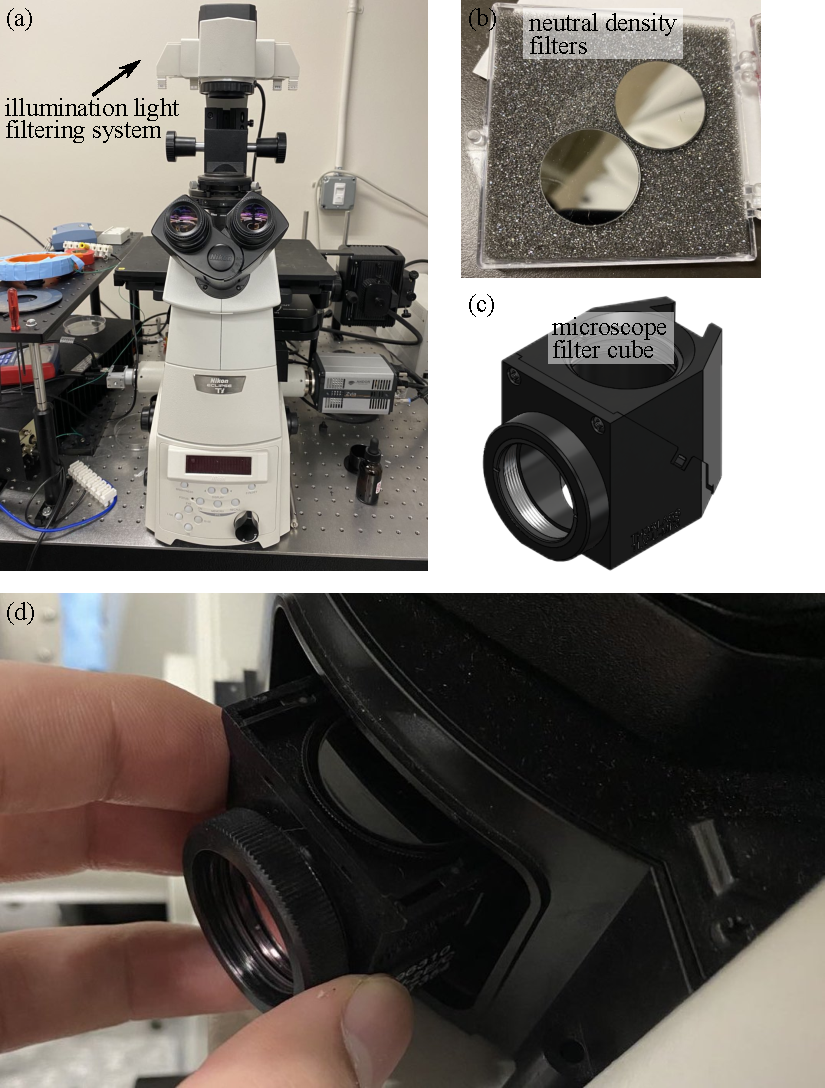
\includegraphics[width=4in]{figs/5-GNF/3.pdf}
\caption[Spatial and Temporal Correlation Functions in Active Turbulence]
{
\textbf{Spatial and temporal correlations functions of density and velocity in active turbulence.}
(a) Two-point density correlations at different bacterial volume fractions $\phi$. Radial position $r$ is normalized by the average length of bacteria $l_b = 3$ $\mu$m.
(b) Density autocorrelations at different $\phi$. Time $t$ is normalized by the characteristic swimming time of bacteria $\tau_b = 0.2$ s.
(c) Two-point velocity correlations at different $\phi$.
(d) Velocity autocorrelations at different $\phi$. $\phi$ ($\%$) of different curves are indicated in (a).
(e) Density and velocity correlation lengths, $\lambda$, versus $\phi$.
(f) Density and velocity correlation times, $\tau$, versus $\phi$.
The error bars in (e) and (f) represent the standard deviations of measurements over 3 independent experiments.
}
\label{fig:spatiotemporal-correlations}
\end{center}
\end{figure}

The correlation length $\lambda$ and correlation time $\tau$ are determined when the corresponding normalized correlation functions decay to $1/e$ (Fig.~\ref{fig:spatiotemporal-correlations}c, f). Figure~\ref{fig:spatiotemporal-correlations}c shows the density correlation lengths at different $\phi$, which characterize the scale of density inhomogeneities in suspensions.
$\lambda$ is small at low $\phi$, gradually increases with $\phi$ and reaches a plateau of $\sim 5l_b$ in high-concentration bacterial suspensions of $\phi > \phi_c = 3.2\%$, where $l_b=3$ $\mu$m is the average length of bacterial body. The velocity correlation length follows the exact same trend and also saturates when $\phi > \phi_c$. Such a quantitative similarity indicates the direct coupling between density fluctuations and collective turbulent flows, a feature we shall examine in much more details later. In the fully-developed turbulent regime above $\phi_c$, the velocity correlation length is about twice the density correlation length.
Fig.~\ref{fig:spatiotemporal-correlations}f shows the density and velocity correlation times at different $\phi$. The velocity and density correlation time at low $\phi$ show a large discrepancy. When $\phi > \phi_c=3.5\%$, they plateau at $\sim 6\tau_b$ and $\sim 4\tau_b$, respectively, where $\tau_b=0.2$ s is the characteristic time scale of \textit{E. coli} swimming.
% I don't know how to interpret the large difference in \tau at low concentration. It may be due to the dominanace of illumination light at low concentration.


\begin{figure}[!p]
\begin{center}
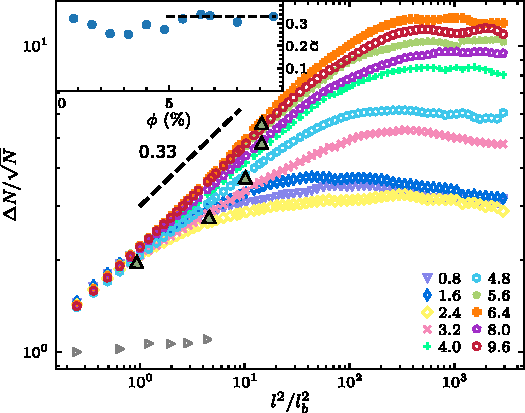
\includegraphics[width=4.5in]{figs/5-GNF/4.pdf}
\caption[Giant Number Fluctuations in Active Turbulence]
{
Density fluctuations of bacterial suspensions of different volume fractions $\phi$. The standard deviation of bacterial number $\Delta N$ in a subsystem of length $l$ as a function of the area of the subsystem $l^2$. $\Delta N$ is normalized by the length of the subsystem $l$, which is proportional to the square root of bacterial number in the subsystem $\sqrt N$. $l$ is presented in a dimensionless form, $\tilde{l} = l/l_b$, where $l_b = 3$ $\mu$m is the average length of bacteria. Dark green triangles indicate the density correlation lengths $\lambda(\phi)$ from Fig.~\ref{fig:spatiotemporal-correlations}e. The black dashed line indicates a power-law scaling of 0.33.
Inset: Scaling exponent $\alpha$ versus $\phi$. $\alpha$ are extracted by fitting the experimental data from 0.3$l_b$ to $\lambda(\phi)$. The dashed line in the inset indicates the theoretical prediction of $\alpha=1/3$.
}
\label{fig:GNF}
\end{center}
\end{figure}

We further examine GNF by calculating the standard deviation of bacterial number $\Delta N$ and the mean bacterial number $N$ in subsystems of increasing sizes. The normalized $\Delta N$ as a function of rescaled subsystem size $\tilde{l}^2=l^2/l_b^2$ for bacterial suspensions of different $\phi$ is plotted in Fig.~\ref{fig:GNF}, where $l$ is the side length of square subsystems.
Note that the area of the subsystem $l^2$ is linearly proportional to mean particle number $N$ at a given $\phi$. At small length scales, when $l\le\lambda_n$, bacterial suspensions of all volume fractions examined in this study (0.8\% to 9.6\%) exhibit GNF, with $\Delta N$ increasing with subsystem size $l^2$. When the size of subsystems is much larger than the density correlation length $\lambda$, the giant fluctuation diminishes due to the spatial average over multiple dense and dilute regions.

The degree of GNF can be quantified by the scaling exponent $\alpha$ following $\Delta N/\sqrt{N} \sim N^\alpha$. $\alpha=0$ for equilibrium systems obeying the central limit theorem, whereas the upper bound $\alpha = 0.5$ corresponds to a system with maximal density fluctuations.
We extract $\alpha$ by fitting the experimental curves with power-law relations only below the density correlation length $\lambda$. The inset of Fig.~\ref{fig:GNF} shows $\alpha$ as a function of $\phi$.

At all volume fractions, $\alpha$ takes a value of $0.30 \pm 0.03$. Notably, at high volume fractions, when $\phi \geq \phi_h = 6.4\%$, $\alpha$ approaches a narrower plateau of $0.33 \pm 0.01$.

The plateau value quantitatively agrees with the theoretical prediction of $\alpha = 1/3$ for 3D suspensions of polar-ordered self-propelled particles with hydrodynamic interactions \cite{Simha2002}. As such, our experiments provide the first quantitative verification of the theory of GNF in 3D wet active fluids.

The observation of GNF at volume fractions lower than $\phi_c$ suggests that even in a dilute suspension below the turbulent transition, bacteria swim in a correlated fashion, in qualitative agreement with the prediction of the kinetic theory \cite{Stenhammar2017}.


\begin{figure}[!p]
\begin{center}
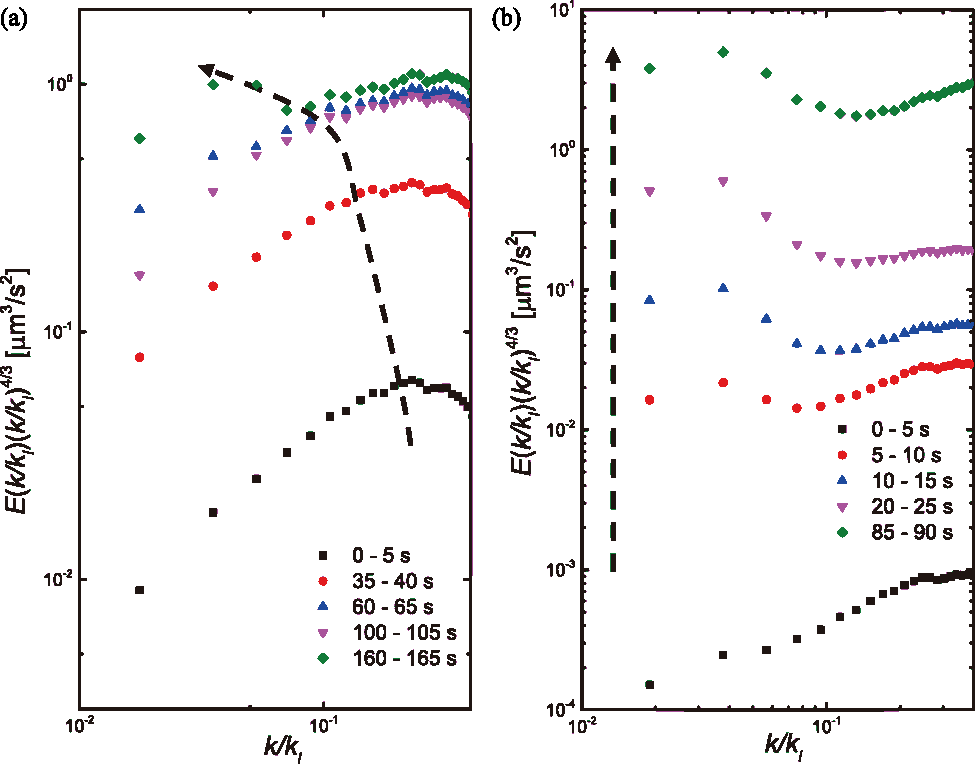
\includegraphics[width=4.5in]{figs/5-GNF/5.pdf}
\caption[Energy Spectra in Active Turbulence]
{
Energy spectra $E(k)$ of bacterial suspensions of different volume fractions $\phi$. Shaded region indicates the range over which the scaling exponent $\beta$ is fitted. The black dashed line indicates a power-law scaling of $-3$. The red dashed line is a fitting of $E(k)$ at $\phi=0.8\%$ using Eq.~\ref{eq:energy-spectra}. In the fitting, the bacterial number density $n=\phi V_b$ and the dipole length $l_d = 1.9$ $\mu$m are from experiments, whereas the dipole strength $\kappa = 100$ $\mu$m$^3$/s and the regularization length $\epsilon = 14$ $\mu$m are taken as fitting parameters. In comparison, $\kappa = 300.8$ $\mu$m$^3$/s from experiments (see text).
Inset: Scaling exponent of $E(k)$, $\beta$, as a function of $\phi$. Dashed line indicates $\beta = 3.3$.
}
\label{fig:energy-spectra}
\end{center}
\end{figure}


\subsection{Energy Spectra}
Similar to GNF, the velocity field of active turbulence also shows scale-dependent structures, which are often characterized by the energy spectrum of turbulent flows, $E(k)$. $E(k)$ measures the kinetic energy density at different scales in terms of wavenumber $k = 2\pi/l$. It is related to the mean kinetic energy density by $\langle \bm{v}^2 \rangle/2 = \langle v_x^2 + v_y^2 \rangle/2 = \int_0^\infty E(k)dk$. Figure~\ref{fig:energy-spectra} shows $E(k)$ of bacterial suspensions at different $\phi$. In the dilute suspension of $\phi = 0.8 \%$, $E(k)$ is independent of $k$ in the small $k$ limit and then decreases at high $k$. The oscillation observed at high $k$ likely arises from PIV errors due to the small number of bacteria in each PIV box of low-$\phi$ suspensions. With increasing $\phi$, $E(k)$ at small $k$ increases sharply. In the turbulent regime at high $\phi$, the kinetic energy is concentrated at scales much larger than the size of single bacteria, even though the turbulent flow is entirely driven by the swimming of single bacteria. The overall trend of $E(k)$ with increasing $\phi$ qualitatively agrees with the results from large-scale particle simulations \cite{Saintillan2012,Bardfalvy2019}.

$E(k)$ of low-$\phi$ suspensions with uncorrelated pusher swimmers has been predicted \cite{Bardfalvy2019}
\begin{equation}
\label{eq:energy-spectra}
E(k) = 4\pi n \kappa^2 \left[ \frac{1}{3} + \frac{\cos(kl_d)}{(kl_d)^2} - \frac{\sin(kl_d)}{(kl_d)^3} \right] \frac{\epsilon^4k^2}{l_d^2} K_2^2(k\epsilon),
\end{equation}
where $n$ is the number density of bacteria, $\kappa$ is the dipole strength and $l_d$ is the dipolar length of \textit{E. coli}. $\epsilon$ is the distance for the regularization of the dipolar flow field. $K_2$ is the modified Bessel function of the second kind.
The fitting of Eq.~\ref{eq:energy-spectra} agrees well with our experimental $E(k)$ at low $\phi$ in the small $k$ limit (Fig.~\ref{fig:energy-spectra}). Particularly, Eq.~\ref{eq:energy-spectra} dictates that $E(k)$ is flat as $k \to 0$, a key feature confirmed by our experiments. A simple dimensional analysis can show that the plateau $E(k)$ at the small $k$ follows $\lim_{k \to 0}E(k) \sim n \kappa^2$ for uncorrelated swimmers of density $n$. The dipole strength can be estimated as $\kappa = Fl_d/\eta = \xi v_0 l_d/\eta = 300.8$ $\mu$m$^3$/s, where $\eta$ is the viscosity of the buffer. $\xi$ is the drag coefficient of a bacterial body orientated along its major axis, which can be calculated based on the body geometry $\xi = 3\pi\eta w_b \left[1-(1-l_b/w_b)/5\right]$ \cite{Magariyama2002}. $l_d = 1.9$ $\mu$m is taken from direct measurements \cite{Drescher2011}. Thus, $\lim_{k \to 0}E(k) \approx 7 \times 10^2$ $\mu$m$^3$/s, within the same order of magnitude of our experiments. The discrepancy between Eq.~\ref{eq:energy-spectra} and experiments at large $k$ may arise from the strong bacterial correlation at small length scales as shown by density fluctuations as well as the PIV errors.


We also extract the scaling exponent $\beta$ of $E(k) \sim k^{-\beta}$ by fitting the energy spectra at intermediate $k$, where a significant change of $E(k)$ with $\phi$ occurs and $E(k)$ exhibits good power-law relations. $\beta$ increases with $\phi$ and saturates around 3 at high $\phi > \phi_c$ (Fig.~\ref{fig:energy-spectra} inset). The saturated scaling exponent quantitatively agrees with previous experimental results obtained from the active turbulence of high-concentration sperm suspensions and \textit{B. subtilis} suspensions at large $k$ \cite{Creppy2015, Wensink2012}. At small $k$, $E(k)$ reported in Ref.~\cite{Wensink2012} decreases with decreasing $k$ and exhibits a non-monotonic trend, different from the result in this work. Such discrepancy is attributed to the confined geometry used in \cite{Wensink2012}, which limits the size of turbulent vortices and thus leads to a decrease of $E(k)$ at small $k$ \cite{Guo2018}. The large system size of $L = 140$ $\mu$m of our experiments allows us to probe the small $k$ limit predicted by theories and simulations without the influence of system boundaries.

Although the scaling in the small $k$ limit is strongly affected by the system size, the scaling in the large $k$ limit seems to be universal with $\beta \approx 3$ from different experiments. To the best of our knowledge, no theoretical prediction has been made on this universal scaling behavior for 3D active turbulence. Giomi investigated the energy spectra of 2D active nematics by combining numerical simulations with mean-field theories and showed $E(k) \sim k^{-4}$ in the large $k$ limit \cite{Giomi2015}.
The result has also been confirmed recently by a hydrodynamic theory \cite{Alert2020}. For isotropic turbulence in $d$ dimension, the energy spectra can be written as $E(k) = C_d k^{d-1} \langle \mathbf{v}(\mathbf{k})\cdot \mathbf{v}(-\mathbf{k})\rangle_{k = |\mathbf{k}|}$ \cite{Wensink2012,Bardfalvy2019},
where $C_d k^{d-1}$ is the surface area of $(d-1)$-sphere and $\langle \mathbf{v}(\mathbf{k})\cdot \mathbf{v}(-\mathbf{k})\rangle_{k = |\mathbf{k}|}$ is the Fourier transform of the velocity-velocity spatial correlation function. If the velocity correlation function for 2D active nematics is qualitatively similar to that of 3D bacterial suspensions independent of the dimensionality of systems, the mean-field theory would then predict a scaling of $E(k) \sim k^{-3}$, consistent with experimental observations. Such a hypothesis, although intriguing, is certainly non-trivial and needs further theoretical investigation.

\begin{figure}[!p]
\begin{center}
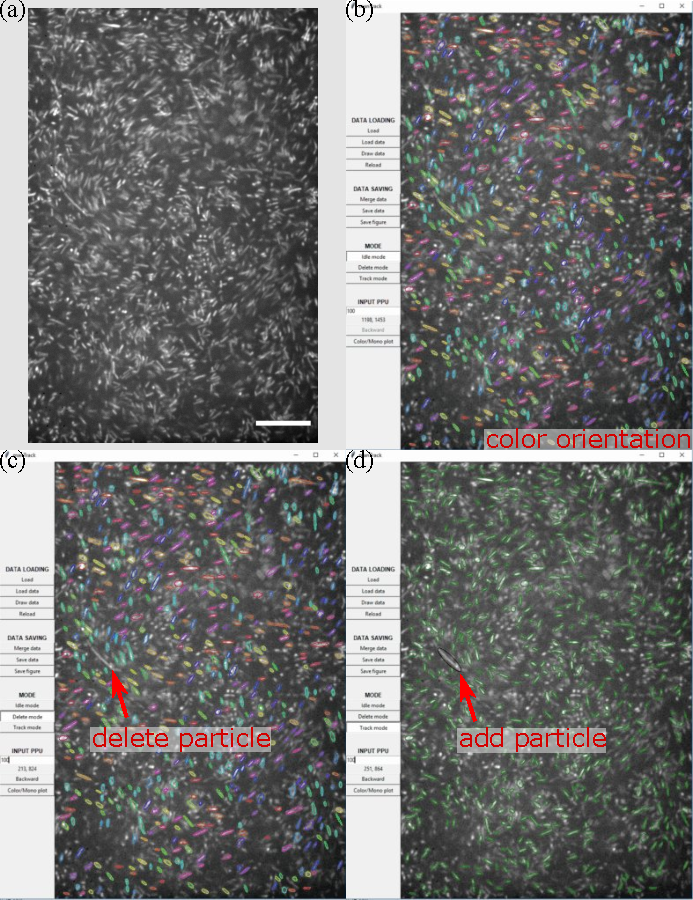
\includegraphics[width=4in]{figs/5-GNF/6.pdf}
\caption[The Coupling between GNF and Kinetic Energy Spectra]
{
The coupling between density fluctuations and kinetic energies in the steady state.
(a) Energy spectra $E(k)$ plotted against number density fluctuations $\Delta N$ at each corresponding length scale for bacterial suspensions of different volume fractions $\phi$. Gray symbols are used for low-$\phi$ suspensions without active turbulence. The black dashed line is a polynomial fitting of the master curve, serving as a guide for the eye. The black arrow indicates the direction of increasing lengths.
(b) Correlation of local density fluctuations and kinetic energies $C$ as a function of $\phi$. $C$ is averaged over 1000 frames in steady state, and the error bars represent the standard deviations. Inset: Density fluctuation and kinetic energy fields in a bacterial suspension of $\phi = 4.8\%$.
}
\label{fig:GNF-energy-spectra-correlation}
\end{center}
\end{figure}


\subsection{Density-Flow Coupling}

Both GNF and energy spectra probe the scale dependence of active turbulence. The former measures density fluctuations at different scales, whereas the latter considers flow energies across scales. Although both properties have been extensively studied, the coupling between the two has not been explicitly examined so far.
The GNF curves and energy spectra shown in Fig.~\ref{fig:GNF} and \ref{fig:energy-spectra} show similar characteristics, including the rapid increase at small length scale and plateaus at large length scale. Such similarity suggests that a density-independent correlation between density fluctuations and kinetic energies may exist across all different length scales.
Indeed, when we plot density fluctuations $\Delta N$ against the corresponding kinetic energies $E$ at the same scale in Fig.~\ref{fig:GNF-energy-spectra-correlation}a, all the $\Delta N$-$E$ pairs fall onto a universal curve over two orders of magnitude in scales extending from the size of single PIV boxes to the vortex size in the turbulent regime, regardless of the specific volume fractions of the samples.
In contrast, $\Delta N$-$E$ shows much larger scattering for low $\phi$ suspensions with random swimming bacteria.
Although it is not surprising that density fluctuations correlate with kinetic energies in general as both measure different aspects of the same active turbulence, the collapse of data from samples of different volume fractions is still quite unexpected.
The results show that the coupling between density fluctuations and turbulent flows occur at every scale of active turbulence in a quantitative same fashion. Such a scale-invariant coupling is independent of the volume fraction of bacterial suspensions. A phenomenological fitting of the universal coupling between density fluctuations and kinetic energy is shown in Fig.~\ref{fig:GNF-energy-spectra-correlation}a by a black dashed line.

To further illustrate such an unusual coupling in real space, we measure the \emph{local} correlation of density fluctuations and kinetic energy at a randomly chosen small scale of $l = 2.5l_b$. The local density fluctuation $\delta N(\mathbf{r},t)$ and local kinetic energy $E(\mathbf{r},t)$ at position $\mathbf{r} = (x,y)$ and time $t$ are extracted from the image intensity field and the PIV velocity field, respectively (Fig.~\ref{fig:GNF-energy-spectra-correlation}b inset).
The normalized correlation between $\delta N(\mathbf{r},t)$ and $E(\mathbf{r},t)$ is then computed at different $\phi$ (Fig.~\ref{fig:GNF-energy-spectra-correlation}b). At low $\phi$ with random swimming bacteria, the correlation is weak fluctuating around zero, which then increases with $\phi$ as bacterial suspensions transition to active turbulence. A constant positive correlation is found in the turbulent regime when $\phi \geq \phi_c$. The real-space measurement provides a concrete example of the coupling between density fluctuations and turbulent flows at small scales.

\begin{figure}[!p]
\begin{center}
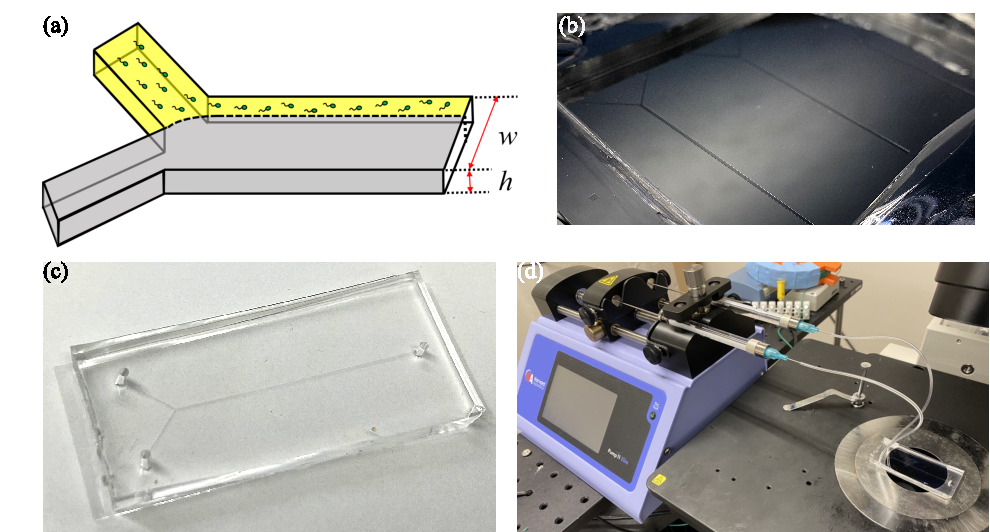
\includegraphics[width=4.5in]{figs/5-GNF/7.pdf}
\caption[Temporal Evolution of $\alpha$, Flow Kinetic Energy $\langle \bm{v}^2 \rangle/2$ and Fraction of Aligned Flow Region $M$]
{
\textbf{Temporal evolution of $\alpha$, flow kinetic energy $\langle \bm{v}^2 \rangle/2$ and fraction of aligned flow region $M$.}
(a) Snapshots of density fluctuation evolution during the transition towards active turbulence, overlaid with velocity fields obtained from PIV analysis. At $t=0$ s, we turn on the illumination light and the bacteria start to gain speed. Times are labeled in corresponding images ($\phi=6.4\%$).
(b) Temporal evolution of scaling exponent $\alpha$, total kinetic energy $E$ and the region fraction of aligned velocity $M$ in the same sample.
}
\label{fig:alpha-kinetics}
\end{center}
\end{figure}


Moreover, we find that the same density-energy coupling also exists in the kinetic process during the transition towards bacterial turbulence. Taking the advantage of the light-powered bacteria, we trigger the onset of bacterial turbulence by suddenly turning on the light illumination on high-$\phi$ bacterial suspensions at $t=0$ \cite{Peng2020}.
The temporal evolution of density fluctuations and turbulent flows in a bacterial suspension of $\phi = 6.4\%$ during the kinetic process is illustrated in Fig.~\ref{fig:alpha-kinetics}a. At $t=0$, the flow velocities are close to 0. The suspension shows no sign of density fluctuations. At $t=40$ s, although the magnitudes of velocities are still small, local alignment of velocity directions can be clearly observed, which gives rise to the characteristic pattern of vortices and jets of active turbulence. Weak density fluctuations start to emerge. At $t=103$ s, the magnitudes of velocities grow significantly and saturate. The suspension reaches the steady state of active turbulence with strong density fluctuations. Note that the response time of individual bacteria is much shorter than the emergence of collective flows.

\begin{figure}[!htbp]
\begin{center}
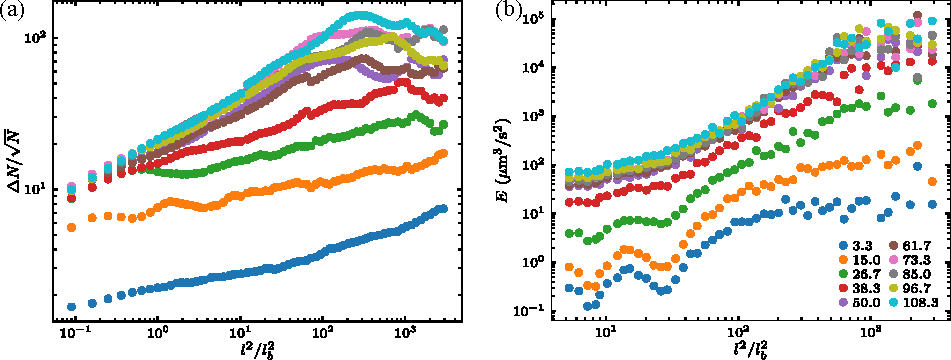
\includegraphics[width=5.5in]{figs/5-GNF/8.pdf}
\caption[Evolution of GNF and Energy Spectra during the Turbulent Transition]
{
\textbf{Evolution of GNF and energy spectra during the turbulent transition.} (a) Number density fluctuations $\Delta N$ and (b) energy spectra $E(k)$ as functions of subsystem size $l^2$ at different times over the turbulence transition of the same bacterial suspension. $\Delta N$ is normalized by the length of subsystems $l$, similar to that in Fig.~\ref{fig:GNF}. $\tilde{l} = l/l_b$. This particular sample has a volume fraction $\phi=6.4$. $t$ is indicated by the legends, in units of seconds.
}
\label{fig:GNF-energy-spectra-kinetics}
\end{center}
\end{figure}

In Fig.~\ref{fig:alpha-kinetics}b, the evolution of the scaling exponent $\alpha$ is shown as a function of $t$. It grows relatively fast at the beginning and shows a saturation at $\sim 60$ s. The growth of both $\alpha$ and the large scale kinetic energy $\langle \bm{v}^2 \rangle/2$ are significantly delayed compared with the formation of collective flows, which is quantified by the area fraction of the regions with strong alignment of local velocities $M$ \cite{Peng2020}.
The finding provides strong experimental support to an important prediction of the kinetic theory of active fluids \cite{Saintillan2008a,Saintillan2008b}, where the density fluctuation arises due to the nonlinear coupling between collective flows and particle densities. At the onset of hydrodynamic instability in the linear regime, when velocities are largely aligned but flow strength is low, GNF is not very pronounced, as confirmed by our experiments at early times.

\begin{figure}[!p]
\begin{center}
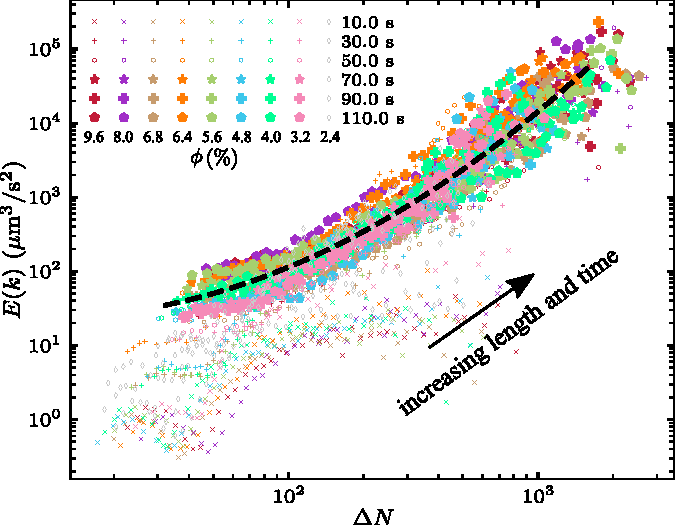
\includegraphics[width=4.5in]{figs/5-GNF/9.pdf}
\caption[Density Flow Coupling during the Transition towards Active Turbulence]
{
\textbf{Density flow coupling during the transition towards active turbulence.}
Kinetic energy $E(k)$ at various length scales is plotted against number fluctuations $\Delta N$ at corresponding length scales for bacterial suspensions at volume fractions ranging from 2.4\% to 9.6\% at different times. Different colors indicate samples of different volume fractions. The size and the shape of the markers indicate the time. Small markers stand for early times and large markers stand for late times. The black dashed line is the same master curve as shown in Fig.~\ref{fig:GNF-energy-spectra-correlation}a. In this plot, length scale and time are hidden variables, and their direction of evolving is indicated by a black arrow.
}
\label{fig:GNF-energy-spectra-correlation-transient}
\end{center}
\end{figure}

By comparing the temporal evolution of both GNF and energy spectra during the turbulence transition as shown in Fig.~\ref{fig:GNF-energy-spectra-kinetics}a and b, we find that they are analogous in at least two ways. First, both quantities reach a saturation at $\sim 60$ s. Second, both quantities grow faster at large length scales. Such analogies indicate that GNF and kinetic energy are  closely coupled not only in the steady state of active turbulence, but also during the transient state in the transition to active turbulence.
Motivated by this observation, we plot $\Delta N$ and $E(k)$ in the same axis for samples of different volume fractions, at different times and length scales in Fig.~\ref{fig:GNF-energy-spectra-correlation-transient}. Indeed, when $\phi>\phi_c$, all the data at different $t$, $\phi$ and length scale $l$ collapse into the same master curve obtained from the steady-state measurements. These kinetic measurements further suggest that the rise of GNF is governed by the kinetic energy at each corresponding scale.



\section{Conclusion}
We have conducted systematic experiments measuring density fluctuations and energy spectra of 3D bacterial suspensions over a wide range of concentrations in both steady and transient states. We illustrated the scaling behavior of giant number fluctuations in bulk bacterial suspensions and showed that such a scaling persisted at small scales even in low-concentration suspensions well before the transition to active turbulence. The finding provided new experimental evidence on the existence of local spatial and temporal correlations between bacteria in dilute suspensions due to the long-range hydrodynamic interactions unique to 3D wet active fluids. In addition, we also examined the energy spectra of bacterial suspensions of different concentrations and showed the spectral properties of the active turbulence of dense bacterial suspensions in the bulk limit. Lastly, by comparing density fluctuations and energy spectra at different scales, we revealed an unexpected coupling between density fluctuations and kinetic energies across more than one order of magnitude of length scales from the scale of single bacteria up to the size of the system. We further showed that such a density-independent and scale-invariant coupling also dominated the kinetic process during the transition towards bacterial active turbulence.

Our experiments also verified several important theoretical predictions on 3D wet active fluids:
\begin{enumerate}
\item The scaling behavior of density fluctuations observed in our experiments
$$
\Delta N/\sqrt N \sim N^{0.33}
$$
quantitatively agreed with the theoretical prediction on the giant number fluctuations of 3D suspensions of polar-ordered self-propelled particles \cite{Simha2002}.
\item The energy spectra of low-concentration bacterial suspensions measured in our study confirmed the key feature of the predicted energy spectra of uncorrelated pusher swimmers in the small wavenumber limit \cite{Bardfalvy2019}.
\item The delayed onset of density fluctuations uncovered in our experiments supported the central prediction of the kinetic theories on the nonlinear development of the hydrodynamic instability of pusher suspensions \cite{Saintillan2008a, Saintillan2008b}.
\end{enumerate}
Thus, our study provided a comprehensive experimental benchmark on the density fluctuations and energy spectra of bulk bacterial suspensions and shed new light onto the emergent dynamics of 3D wet active fluids.
